\documentclass[9pt,twocolumn,twoside]{styles/osajnl}
\usepackage{fancyvrb}
\journal{i524} 

\title{\LaTeX\ Template for Preparing a Paper or Report for I524}

\author[1,2,3]{John Smith}
\author[2]{Alice Smith}
\author[1]{Bruce Wayne}
\author[1,*]{Gregor von Laszewski}

\affil[1]{School of Informatics and Computing, Bloomington, IN 47408, U.S.A.}
\affil[2]{School of Science, University of Technology, 2000 J St. NW, Washington DC, 20036}
\affil[3]{School of Optics, University of Technology, 2000 J St. NW, Washington DC, 20036}

\affil[*]{Corresponding authors: laszewski@gmail.com}

\dates{project-000, \today}

\ociscodes{Cloud, I524}

% replace this with your url in github/gitlab
\doi{\url{https://github.com/cloudmesh/classes/blob/master/docs/source/format/report/report.pdf}}


\begin{abstract}
This template can be used to prepare a research article for I524. Note
that this template can be run from your own \TeX\ system or within the
cloud-based \href{https://www.overleaf.com}{Overleaf} system or \href{https://www.sharelatex.com/}
{Sharelatex} systems.\newline
\end{abstract}

\setboolean{displaycopyright}{true}

\begin{document}

\maketitle

\section{Introduction}

This template is designed to assist with creating an article for
I524. The page length is typically done without images. Thus if you
have images in your report, please add additional content to offset
the space captured by images. We do not check exactly, so there is no
reason to contact us if you are a paragraph short, but if you are half
a page short you may add quality content.

\section{Chance for Publishing a Paper}

If this work can lead to a publishable paper, you could engage with
the course instructor as coauthor to work more closely with him/them.
This however requires that the paper be worked on in a regular basis
and that timely contributions from the instructor can be integrated.
Hence this is going to be a significant effort and you need to decide
if you like to conduct this. Naturally the project must be suitable
for such an activity. It may even be that some projects may be
combined.

In such cases if the work is sufficient for publication submission, an
A+ for the class could be considered. It will be however a lot of
work. The length of such a paper is typically 10-12 high quality pages
including figures and references. We may elect for the final
submission to use a different LaTeX style. As Gregor is an expert in
this, changing the format will be simple.

\section{Examples of Article Components}
\label{sec:examples}

The sections below show examples of different article components.

\section{Figures and Tables}

It is not necessary to place figures and tables at the back of the
manuscript. Figures and tables should be sized as they are to appear
in the final article. Do not include a separate list of figure
captions and table titles.

Figures and Tables should be labelled and referenced in the standard
way using the \verb|\label{}| and \verb|\ref{}| commands.

\subsection{Sample Figure}

Figure \ref{fig:false-color} shows an example figure.

\begin{figure}[htbp]
\centering
\fbox{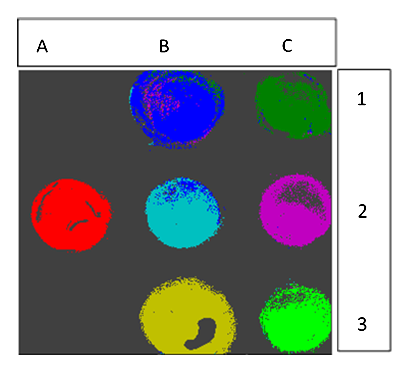
\includegraphics[width=\linewidth]{images/sample}}
\caption{False-color image, where each pixel is assigned to one of seven reference spectra.}
\label{fig:false-color}
\end{figure}

\subsection{Sample Table}

Table \ref{tab:shape-functions} shows an example table.

\begin{table}[htbp]
\centering
\caption{\bf Shape Functions for Quadratic Line Elements}
\begin{tabular}{ccc}
\hline
local node & $\{N\}_m$ & $\{\Phi_i\}_m$ $(i=x,y,z)$ \\
\hline
$m = 1$ & $L_1(2L_1-1)$ & $\Phi_{i1}$ \\
$m = 2$ & $L_2(2L_2-1)$ & $\Phi_{i2}$ \\
$m = 3$ & $L_3=4L_1L_2$ & $\Phi_{i3}$ \\
\hline
\end{tabular}
  \label{tab:shape-functions}
\end{table}

\section{Sample Equation}

Let $X_1, X_2, \ldots, X_n$ be a sequence of independent and
identically distributed random variables with $\text{E}[X_i] = \mu$
and $\text{Var}[X_i] = \sigma^2 < \infty$, and let

\begin{equation}
S_n = \frac{X_1 + X_2 + \cdots + X_n}{n}
      = \frac{1}{n}\sum_{i}^{n} X_i
\label{eq:refname1}
\end{equation}

denote their mean. Then as $n$ approaches infinity, the random
variables $\sqrt{n}(S_n - \mu)$ converge in distribution to a normal
$\mathcal{N}(0, \sigma^2)$. 

\section{Sample Algorithm}

Algorithms can be included using the commands as shown in algorithm
\ref{alg:euclid}.

\begin{algorithm}
\caption{Euclid’s algorithm}\label{alg:euclid}
\begin{algorithmic}[1]
\Procedure{Euclid}{$a,b$}\Comment{The g.c.d. of a and b}
\State $r\gets a\bmod b$
\While{$r\not=0$}\Comment{We have the answer if r is 0}
\State $a\gets b$
\State $b\gets r$
\State $r\gets a\bmod b$
\EndWhile\label{euclidendwhile}
\State \textbf{return} $b$\Comment{The gcd is b}
\EndProcedure
\end{algorithmic}
\end{algorithm}

\begin{algorithm}
\caption{Python example}\label{alg:python}
\begin{quote}
\begin{Verbatim}[numbers=left]
for i in range(0,100):
  print i
\end{Verbatim}
\end{quote}
\end{algorithm}

\section{Reference Management}

The best programs to manage your references is jabref or emacs. You
can edit the references and verify them with them for format
errors. To cite them use the citation key. You can add multiple bib
files to the bibliography command separated by comma.

\noindent Add citations with the cite command. See
\cite{las14cloudmeshmultiple} for an example on how to use multiple
clouds. In \cite{www-i524} we list the class content.

Here a test of a citation with an underscore in the url \cite{www-underscore}.

\section{Supplemental Material}

You can include an appendix with important information and additional
figures if needed. However they must be referenced and follow the same
guidelines as in the main text.  All materials must be associated with
a figure, table, or equation or be referenced in the results section
of the manuscript.  (1) 2D and 3D image files and video must be
labeled “Visualization,” not “Movie,” “Video,” “Figure,” etc.  (2)
Machine-readable data (for example, csv files) must be labeled “Data
File.”  Number data files and visualizations consecutively, e.g.,
“Visualization 1, Visualization 2….”  (3) Large datasets or code files
must be placed in github/gitlab.  Such items should be mentioned in
the text as either “Dataset” or “Code,” as appropriate, and also be
cited in the references list. Appropriate citations in jabref as Misc
need to be created.

\section*{Acknowledgements}

Funding information should be listed in this section. Please evaluate
if you like to list your employer that may have funded your activities
here.  If you receive grants or project numbers, as shown in the
example.  This work was in part supported by National Science
Foundation (NSF) (1234567, 891012345) (These numbers are invented)

The acknowledgments may also contain any information that is not
related to funding:

The authors thank H. Haase, C. Wiede, and J. Gabler for technical
support.


% Bibliography

\bibliography{references}
 
\section*{Author Biographies}
\begingroup
\setlength\intextsep{0pt}
\begin{minipage}[t][3.2cm][t]{1.0\columnwidth} % Adjust height [3.2cm] as required for separation of bio photos.
  \begin{wrapfigure}{L}{0.25\columnwidth}
    
\includegraphics[width=0.25\columnwidth]{images/john_smith.eps}
  \end{wrapfigure}
  \noindent
  {\bfseries John Smith} received his BSc (Mathematics) in 2000 from
  The University of Maryland. His research interests include lasers
  and optics. 
\end{minipage}
\begin{minipage}[t][3.2cm][t]{1.0\columnwidth} % Adjust height [3.2cm] as required for separation of bio photos.
  \begin{wrapfigure}{L}{0.25\columnwidth}
    
\includegraphics[width=0.25\columnwidth]{images/alice_smith.eps}
  \end{wrapfigure}
  \noindent
  {\bfseries Alice Smith} received her BSc (Mathematics) in 2000 from
  The University of Maryland. Her research interests also include
  lasers and optics. 
\end{minipage}
\begin{minipage}[t][3.2cm][t]{1.0\columnwidth} % Adjust height [3.2cm] as required for separation of bio photos.
  \begin{wrapfigure}{L}{0.25\columnwidth}
    
\includegraphics[width=0.25\columnwidth]{images/alice_smith.eps}
  \end{wrapfigure}
  \noindent
  {\bfseries Bruce Wayne} received his BSc (Aeronautics) in 2000 from
  Indiana University. His research interests include lasers and optics.
\end{minipage}
\endgroup

\newpage

\appendix

\section{Work Breakdown}

The work on this project was distributed as follows between the
authors:

\begin{description}

\item[John Smith.] Explored the deep mathematical knowledge needed for
  this paper and taught it to the other authors.

\item[Alice Smith.] She explored the world of Oz and was instrumental
  to work on the deployment of hadoop.

\item[Bruce Wayne.] He did not contribute at all to this paper and
  flew around to safe the world.  

\end{description}

\section{Report Checklist}

\begin{itemize}
\renewcommand{\labelitemi}{\scriptsize$\square$} 
\item Have you written the report in word or LaTeX in the specified
  format?
\item Have you included the report in github/lab?
\item Have you specified the names and e-mails of all team members in
  your report. E.g. the username in Canvas?
\item Have you included the HID of all team members?
\item Does the report have the project number added to it?
\item Have you included all images in native and PDF format in gitlab
  in the images folder?
\item Have you added the bibliography file in bibtex format?
\item Have you submitted an additional page that describes who did
  what in the project or report?
\item Have you spellchecked the paper?
\item Have you made sure you do not plagiarize?
\item Have you made sure that the important directories are all lower
  case and have no underscore or space in it?
\item Have you made sure that all authors have a README.rst in their
  HID github/lab repository?
\item Have you made sure that there is a README.rst in the project
  directory and that it is properly filled out?
\item Have you put a work breakdown in the document if you worked in a
  group?
\end{itemize}

\section{Possible technology paper outline}

The next sections are just some suggestions, your may want to add
sections and subsections as you see fit. Images and references do not
count towards the 2 page length. Please use the \verb|\section|,
\verb|\subsection|, and \verb|\subsubsection| commands in your
paper. do not introduce hardcoded numbers. Use the \verb|\ref| and
\verb|\label| commands to refer
 to the sections.


\paragraph{Abstract}

Put in the abstract a summary what this paper is about

\paragraph{1. Introduction}

Introduce the technology and provide general useful information.

\paragraph{2. Architecture} 

If applicable include a description about architectural details. This
may include a figure. Make sure that if you copy a figure you put the
\cite{?} in the caption also. Otherwise it is plagiarism.

\paragraph{2.1. API}

comment on the API which could include language bindings

\paragraph{2.2. Shell Access}

If applicable comment on how the tool can be used from the command line

\paragraph{2.3.Graphical Interface}

If applicable comment on if the technology has a GUI

\paragraph{3. Licensing}

Often tools may have different versions, some fre, some for
pay. Comment on this. For example while a tool may offer a comercial
version this version may be too costly for others. Identify especially
the difference between features for free vs commercial tools.

Sometimes you may need to introduce this also in the introduction as
there may be a big difference and without the knowledge you do not
provide the user an adequate introduction.

\paragraph{4. Ecosystem}

Some technologies have a large ecosystem developed around them with
extensions plugins and other useful tools. Identify if they exists and
comment on what they can achieve

provide potentially a mindmap or a figure illustrating how the
technology fits in with other technologies if applicable.

\paragraph{4. Use Cases}

\paragraph{4.1. Use Cases  for Big Data}

Locate and describe major usecases that demonstrate the technology
while focussing on big data related use cases. Make sure you do proper
references with the \cite{?} command. Do not put URLs in the text.

\paragraph {4.2. Other Use Cases}

Some technologies may not just be used for big data, find other makor
use cases from other areas if applicable.  Make sure you do proper
references with the \cite{?} command. Do not put URLs in the text.

\paragraph{5. Educational material}

Put information here how someone would find out more about the
technology. Use important material and do not list hundrets of web
pages, be selective.

\paragraph{6. Conclusion}

Put in some conclusion based on what you have researched

\paragraph{Acknowledgement}

Put in the information for this class and who may sponsor
you. Examples will be given later

\end{document}
